% Médiation et documentation

\subsection{Échanges avec les chercheurs}
La médiation et la rédaction de documentation est un aspect essentiel de l'intégration de l'\ia aux pratiques des chercheurs. Une communication fluide se doit d'exister entre les équipes d'ingénierie et de recherches, pour trouver un équilibre entre les exigences scientifiques et les contraintes techniques et ainsi permettre la réalisation d'outils répondant aux attentes des utilisateurs. Ces allers-retours sont un pilier pour le développement d'outils utiles et utilisés, qui auront un impact réellement positif sur les publics qu'ils ont pour vocation de servir. 
	
    \subsubsection{Séminaires DH}
    Dans le cadre du projet \eida, des séminaires mensuels d'humanités numériques, ou \textit{DH Seminars}, sont organisés à destination de l'équipe. Ces séminaires, donnés par les membres du projet ou par des intervenants extérieurs, permettent à la fois de tenir les chercheurs informés de l'avancement des développements numériques liés à \eida, et de mener des introductions à des outils informatiques pouvant présenter un intérêt pour les membres de l'équipe. Ces séminaires permettent de maintenir le lien entre les ingénieurs et les chercheurs, en créant un espace pour la circulation de l'information autour du développement des outils du projet, et en les accompagnant dans la prise en main d'outils numériques de soutien à la recherche.
    
    Lors des \textit{DH Seminars} de l'année 2022-2023, les membres de l'équipe \eida ont ainsi été introduits, par des chercheurs partenaires ou par les ingénieurs du projets, à des outils pour le traitement et la visualisation des sources de leurs corpus : ont ainsi été présentés des outils pour l'édition numériques des diagrammes astronomiques et pour la visualisation de données, et un séminaire a été dédié à la prise en main du logiciel Gephi\footcite{Gephi}, dédié à la représentation de réseaux. Ces séminaires axés sur des outils spécifiques permettent ainsi de proposer aux chercheurs une introduction guidée à des utilitaires informatiques intéressants.
    
    Les séminaires tournés vers la présentation des outils numériques du projet sont axés sur les éléments auxquels sont confrontés les chercheurs dans leurs pratiques, en éludant les points plus techniques qui concernent exclusivement l'ingénierie. Ainsi, les séminaires présentant les travaux de l'équipe d'ingénierie du projet \eida concernent le développement de la plateforme ou la correction des détections, et offrent aux chercheurs un espace pour exprimer leurs besoins en tant qu'utilisateurs des outils développés, et pour poser leurs questions. À titre d'exemple, la présentation d'\exapi (Annexe \ref{DHSeminar}) donnée lors du séminaire\footnote{Le séminaire a été donné le 13 juin 2023 aux membres de l'équipe \eida pour présenter les développements réalisés lors du stage. Le document fourni en annexe \ref{DHSeminar} est un diaporama utilisé en support de la présentation.} est orientée vers une introduction aux \api et à leur fonctionnement, suivi d'une explication des étapes de la chaîne de traitement automatique des sources, pour donner aux chercheurs une vision plus concrète des échanges et transformations liées aux données qui se produisent en \textit{back end} entre l'envoi d'une numérisation et le retour des annotations. La discussion à l'issue de ce séminaire a été orientée sur les bonnes pratiques en termes de correction de la détection et sur les besoins techniques pour la constitution d'un jeu de données d'entraînement, tâche à laquelle les chercheurs prennent une part active.
	
    \subsubsection{Ateliers d'annotation}
    Dans le contexte d'un projet visant à la création d'un modèle de vision artificielle, les ateliers d'annotation permettent de s'assurer de l'uniformité des données produites par les chercheurs pour l'entraînement, et de créer un espace où peuvent être réunies les équipes de recherche et d'ingénierie pour confronter, dans la pratique, les exigences scientifiques aux possibilités techniques, et apporter des solutions en accord avec les besoins de chaque équipe. Le projet \eida tient ces ateliers en présence des équipes de recherche et d'ingénierie, ainsi que des membres du laboratoire \imagine, chargés du développement des modèles. À l'Observatoire de Paris, les ateliers d'annotations tenus ont portés sur la correction des résultats de l'algorithme de détection, et sur la correction des résultats d'un algorithme de vectorisation proposé par le laboratoire \imagine\footnote{La vectorisation constitue, pour le projet \eida, une étape plus tardive, liée au développement d'une plateforme pour l'édition automatique de diagrammes. Nous expliquons cette démarche dans le chapitre \ref{vectorEdition}.}. Il est proposé aux chercheurs d'effectuer les corrections en temps réel, leur permettant de poser les questions soulevées par la confrontation aux sources et aux performances des outils développés. Les ateliers sont ainsi l'occasion d'établir les bonnes pratiques qui sont ensuite consignées dans des guides d'annotation qui assurent l'uniformité de la démarche de correction, et donc des jeux de données d'entraînement. Cet espace d'échange permet une communication fluide entre les équipes, et évite un cloisonnement du travail qui générerait des données inégales.
    
    Les ateliers d'annotation constituent également une première confrontation des interfaces avec les chercheurs du projet. En tant que premier public de ces interfaces, les chercheurs ont la possibilité de prendre en main les outils développés, et de fournir un retour de leur expérience en tant qu'utilisateurs. Cette confrontation des utilisateurs aux interfaces permet d'ajuster les développements selon les remarques et besoins des membres de l'équipe, enrichissant ainsi l'élaboration de l'interface publique du regard de ceux à qui elle est dédiée.

    
\subsection{Documentation et wiki : penser le réemploi du code}
En parallèle de la communication pour et avec les chercheurs, il est de bonne pratique de rédiger une documentation dédiée aux développeurs. Cette documentation est une forme de médiation autour du code produit. Elle permet d'assurer la continuité entre les différentes personnes impliquée dans le développement, et entre les différents développeurs qui pourraient être amenés à utiliser, modifier, améliorer le code au cours de la vie de l'outil produit. Cette documentation à destination de ce groupe particulier d'utilisateurs prend une importance particulière dans le cadre de la création d'un outil réutilisable, qui doit s'accompagner de l'ensemble des informations nécessaires à l'utilisation du code, de l'installation au déploiement.
	
    \subsubsection{Commentaires dans le code}
    La rédaction de commentaires au sein du code est essentielle pour en permettre la maintenance et le remploi ultérieur. Au-delà des bonnes pratiques pour la lisibilité du code, telles que le nommage explicite des fonctions et des variables ou l'allègement au possible de la structure du code pour son intelligibilité, la rédaction de commentaires permet d'enrichir le code d'explications. 
    
    L'insertion des commentaires permet d'expliciter des éléments précis du code, à la ligne près, pour assurer une lecture fluide par d'autres membres de l'équipe, par des développeurs souhaitant réemployer le code, ou par le développeur lui-même, pour résoudre des \textit{bugs} ou effectuer des modifications. Lors de la conception d'\exapi, des commentaires ont été ajoutés pour expliciter les passages peu intelligibles du code (fig. \ref{fig:commentaire_exapi}), en complément d'une relecture pour vérifier assurer l'absence de redondance et de lignes de code inutiles, et simplifier les fonctions. 
    
    \begin{figure}[h]
   		\begin{lstlisting}[language=Python]
   		# If annotations are generated again, empty annotation file
   		if exists(anno_file):
   		open(anno_file, 'w').close()\end{lstlisting}
   		\caption{Exemple de commentaire dans le code d'\exapi}
   		\label{fig:commentaire_exapi}
    \end{figure}
	
	La rédaction de commentaires permet de s'assurer de l'accessibilité des développements, qui se doivent d'être lisibles pour assurer la fluidité du développement en équipe, et pour être réutilisables. Une documentation rédigée pour accompagner un code de qualité permet d'assurer aux utilisateurs extérieurs comme aux futurs développeurs du projet la possibilité de naviguer le code sans restructuration de celui-ci.

    \subsubsection{Rédaction d'un wiki}
    La rédaction d'une documentation plus globale sur le développement réalisé doit accompagner les commentaires, qui assurent la lisibilité du code à une granularité plus fine. La publication du code d'une application dans un dépôt GitHub pour sa mise à disposition en accès libre peut s'accompagner d'un wiki, constitué de plusieurs pages de documentation en lien avec l'architecture globale de l'outil. Ce wiki permet de mettre à disposition des développeurs un ensemble d'informations liées à l'exploitation du code, nécessaire à l'installation et au déploiement du développement.
    
    \begin{figure}[h]
    	\centering
    	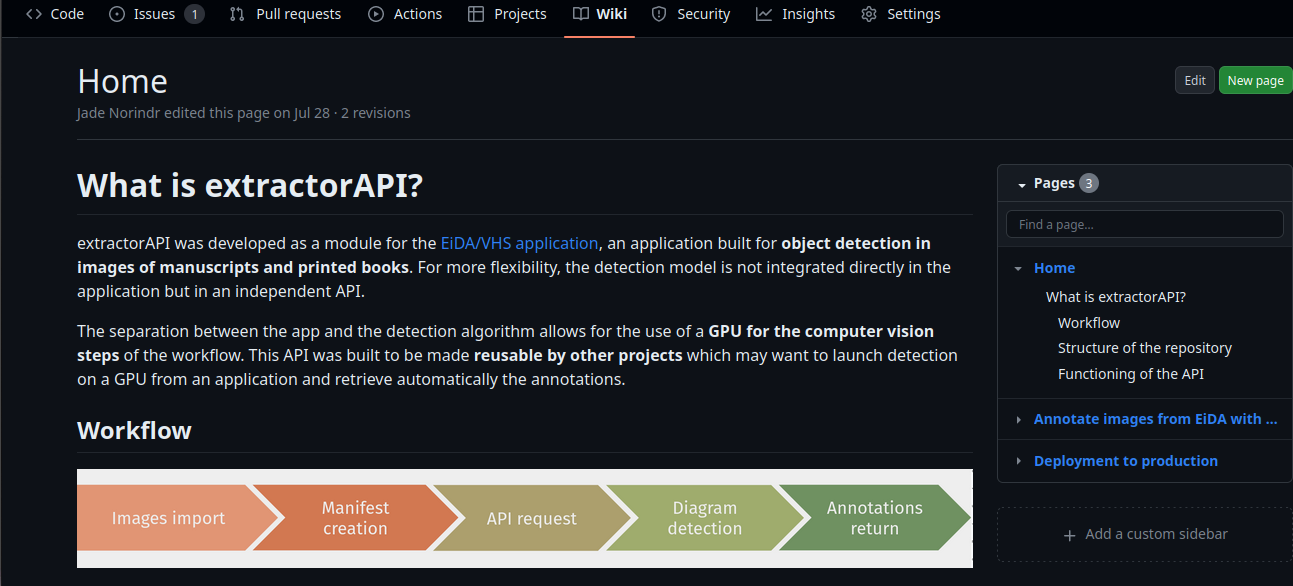
\includegraphics[width=15cm]{images/exapi_wiki.png}
    	\caption{Capture d'écran de la page d'accueil du wiki d'\exapi sur GitHub}
    	\label{fig:exapi_wiki}
    \end{figure}
    
    La rédaction d'une documentation librement accessible en accompagnement du code permet d'expliquer ses fonctions et son architecture globale aux développeurs qui souhaiteraient le réemployer, et d'en documenter des aspects spécifiques nécessaires à son bon fonctionnement. Ainsi, le wiki rédigé pour la publication du code d'\exapi\footcite{ExtractorAPIWiki2023} (fig. \ref{fig:exapi_wiki}), disponible sur GitHub, présente les fonctionnalités de l'\api développée\footnote{En annexe \ref{exapiAnno}, nous avons retranscrit une page rédigée pour le wiki explicitant les interactions entre \exapi et l'application \eida, pour les développeurs qui souhaiteraient l'utiliser en lien avec une application et mettre en place les requêtes de la même manière. L'accent est mis sur le lancement en tâche de fond de la détection, pour éviter l'interruption de l'application en attendant la réponse de l'\api.}, et proposé également une page dédiée au déploiement en production\footcite{DeploymentProductiona}, étape nécessaire pour les développeurs qui souhaiteraient utiliser l'outil. Cette documentation se doit d'être claire, structurée, et de faire référence au code pour permettre sa navigation, et en fluidifier le réemploi par des développeurs extérieurs au projet. À l'inverse des séminaires et documents proposés aux chercheurs, cette documentation est dédiée à un public formé en programmation, et se focalise donc sur les aspects techniques du développement plutôt que sur l'usage scientifique qui peut en être fait.
    
	La documentation et la médiation sont des pratiques inhérentes à la création d'outils numériques, et se doivent d'exister en parallèle des tâches de développement pour assurer un lien avec les équipes scientifiques, mais aussi une transmission au sein des équipes techniques, qui assurent le maintient, l'amélioration et le réemploi du code. Il est ainsi crucial pour le développeur de penser cette documentation en parallèle du travail de programmation pour éviter le cloisonnement entre les différents acteurs d'un projet, mais aussi dans une démarche d'\textit{open source}.
